\begin{frame}%[<+=>]
  \frametitle{Introduction}
\small
  \begin{itemize}[<+->]
    \item Laplace-Young equation model surface tension effects for enclosed liquids.
    \item Combining surface tension, gravity and contact the energy functional for Laplace-Young is:
      \begin{gather*}
       % E(u,\nabla u)
       % =
        \int_\Omega \sqrt{1+|\nabla u|^2} \;d\Omega
        +
        \int_\Omega \frac 12 \kappa u^2 \;d\Omega
        -
        \int_{\partial\Omega} \sigma u \;ds
      \end{gather*}
      \item Where $\kappa$ is the ratio of surface energy to gravitational energy and $u$ is the height of the liquid.

    \item While the weak formulation of the stationary condition is given by:
      \begin{align}
        \label{eq:weak}
       % a(\kappa,\sigma;u,\varphi)
       % =
        \left(\frac{\nabla u}{\sqrt{1+|\nabla u|^2}},
          \nabla \varphi \right)_\Omega
        +
        \kappa\left(u,\varphi\right)_\Omega
        =
        \sigma \left(1,\varphi\right)_{\partial\Omega} 
%        \qquad
%        \forall \varphi\in V
      \end{align}

    \item By specifying the parameter $\sigma=cos(\gamma)$ (where $\gamma$ is the contact angle) along the boundary, the liquid height $u$ can be solved for.
  \end{itemize}
\end{frame}

\begin{frame}[fragile,t]
\tiny
\begin{block}{}
  Instead of explicitly finding the Jacobian, we'll use FEMSystem to finite difference the weak form.
\end{block}

\begin{block}{element\_constraint()}
\begin{semiverbatim}
  for (unsigned int qp=0; qp != n_qpoints; qp++) \{
    Number u = interior_value(0, qp);
    Gradient grad_u = interior_gradient(0, qp);
    \alert<2>{Number K = 1. / sqrt(1. + (grad_u * grad_u));}

    for (unsigned int i=0; i != n_u_dofs; i++) \{
      Fu(i) += JxW[qp] * ((\alert<5>{_kappa * u * phi[i][qp]}) +
               (\alert<2>{K} * \alert<3>{grad_u} * \alert<4>{dphi[i][qp]}));
    \}
  \}
\end{semiverbatim}
\end{block}

\begin{block}{side\_constraint()}
\begin{semiverbatim}
  for (unsigned int qp=0; qp != n_qpoints; qp++) \{
    for (unsigned int i=0; i != n_u_dofs; i++) \{
      Fu(i) -= JxW[qp] * \alert<6>{_gamma * phi[i][qp]};
    \}
  \}
\end{semiverbatim}
\end{block}

\begin{block}{}
   \begin{equation}
     \nonumber
       \left(\frac{\alert<3>{\nabla u}}{\alert<2>{\sqrt{1+|\nabla u|^2}}},
           \alert<4>{\nabla \varphi} \right)_\Omega
         +
         \alert<5>{\kappa\left(u,\varphi\right)_\Omega}
         -
         \alert<6>{\sigma \left(1,\varphi\right)_{\partial\Omega}} 
         =
         0
         \qquad
         \forall \varphi\in V
   \end{equation}
\end{block}

\end{frame}

\frame
{
  \frametitle{Solution}
  \small
  \begin{itemize}[<+->]
    \item An overkill solution containing 200,000 DOFs.
  \end{itemize}
      \begin{figure}[!htb]
        \begin{center}
          \subfigure[2D.]{\label{fig:ly_over_2d}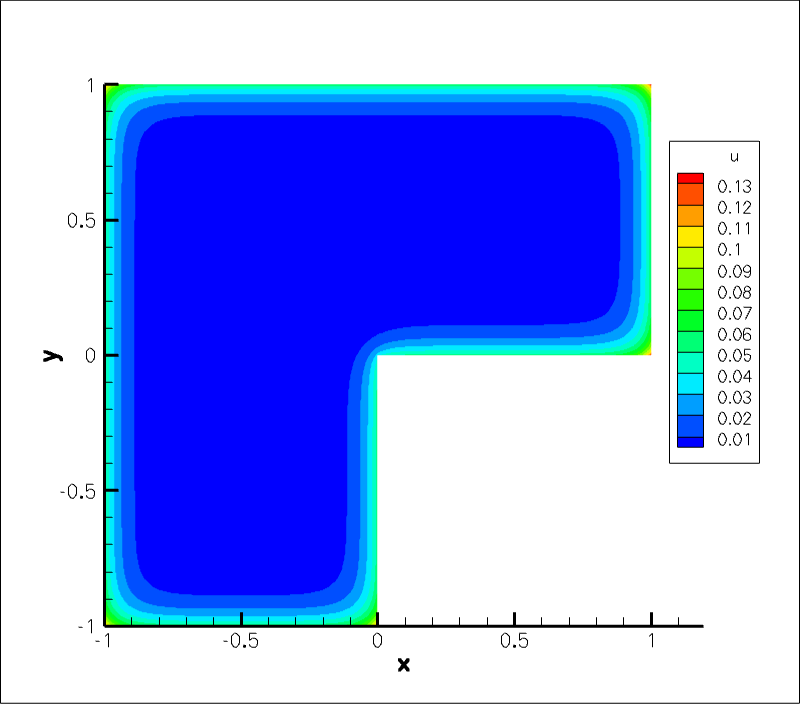
\includegraphics[viewport=40 20 660 650,clip=true,width=.42\textwidth]{figs/ly_over_2d}}
          \subfigure[Contour Elevation.]{\label{fig:ly_over_3d}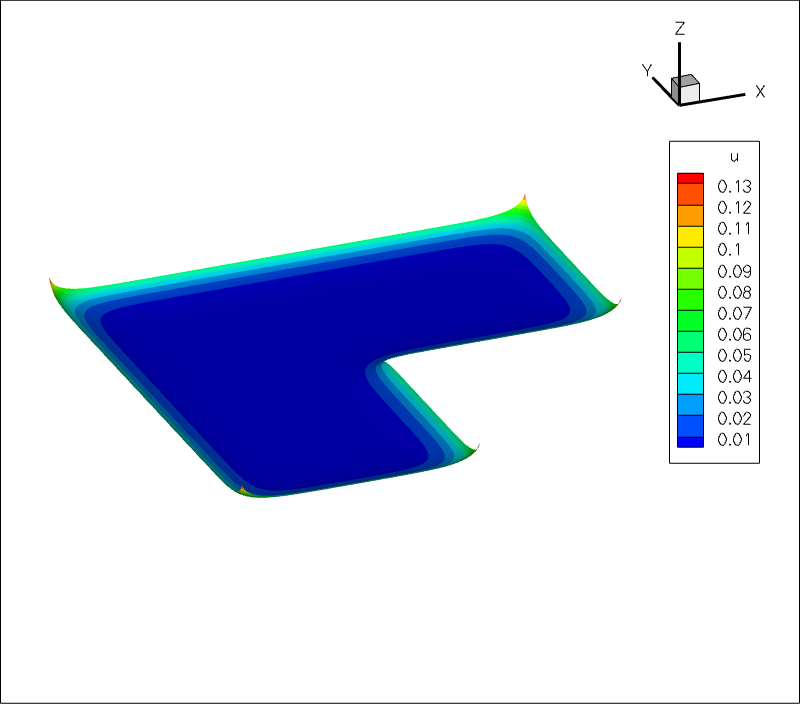
\includegraphics[viewport=50 70 620 550,clip=true,width=.42\textwidth]{figs/ly_over_3d}}
        \label{fig:ly_over}
        \end{center}
      \end{figure}
}

% \frame
% {
%   \frametitle{Redistributed Solution}
%   \begin{itemize}[<+->]
%     \item Using a set of variational smoothing functionals and an error indicator for redistribution the following grid and solution can be obtained.
%       \begin{figure}[!htb]
%         \begin{center}
%           \subfigure[Mesh.]{\label{fig:ly_redist_11_mesh}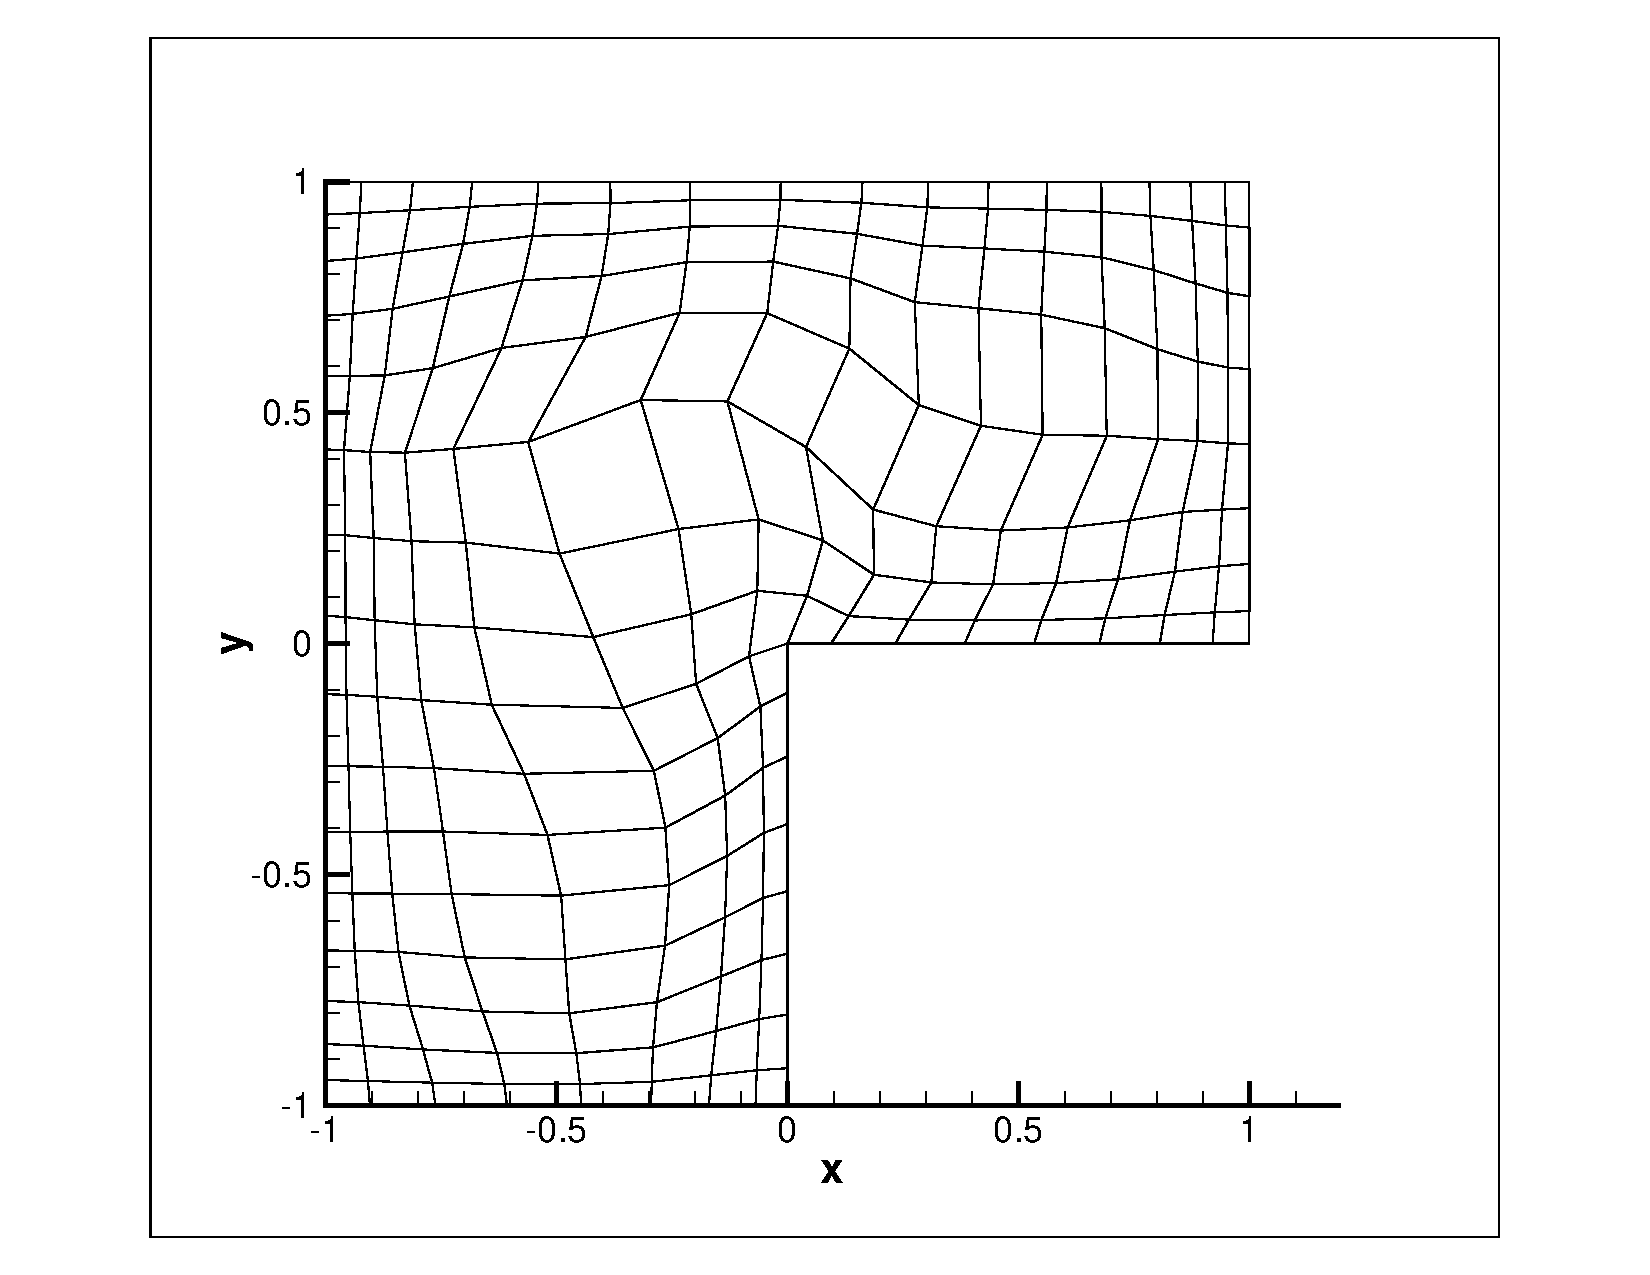
\includegraphics[viewport=110 30 600 550,clip=true,width=.42\textwidth]{figs/ly_redist_14_mesh.pdf}}
%           \subfigure[Solution.]{\label{fig:ly_redist_11_sol}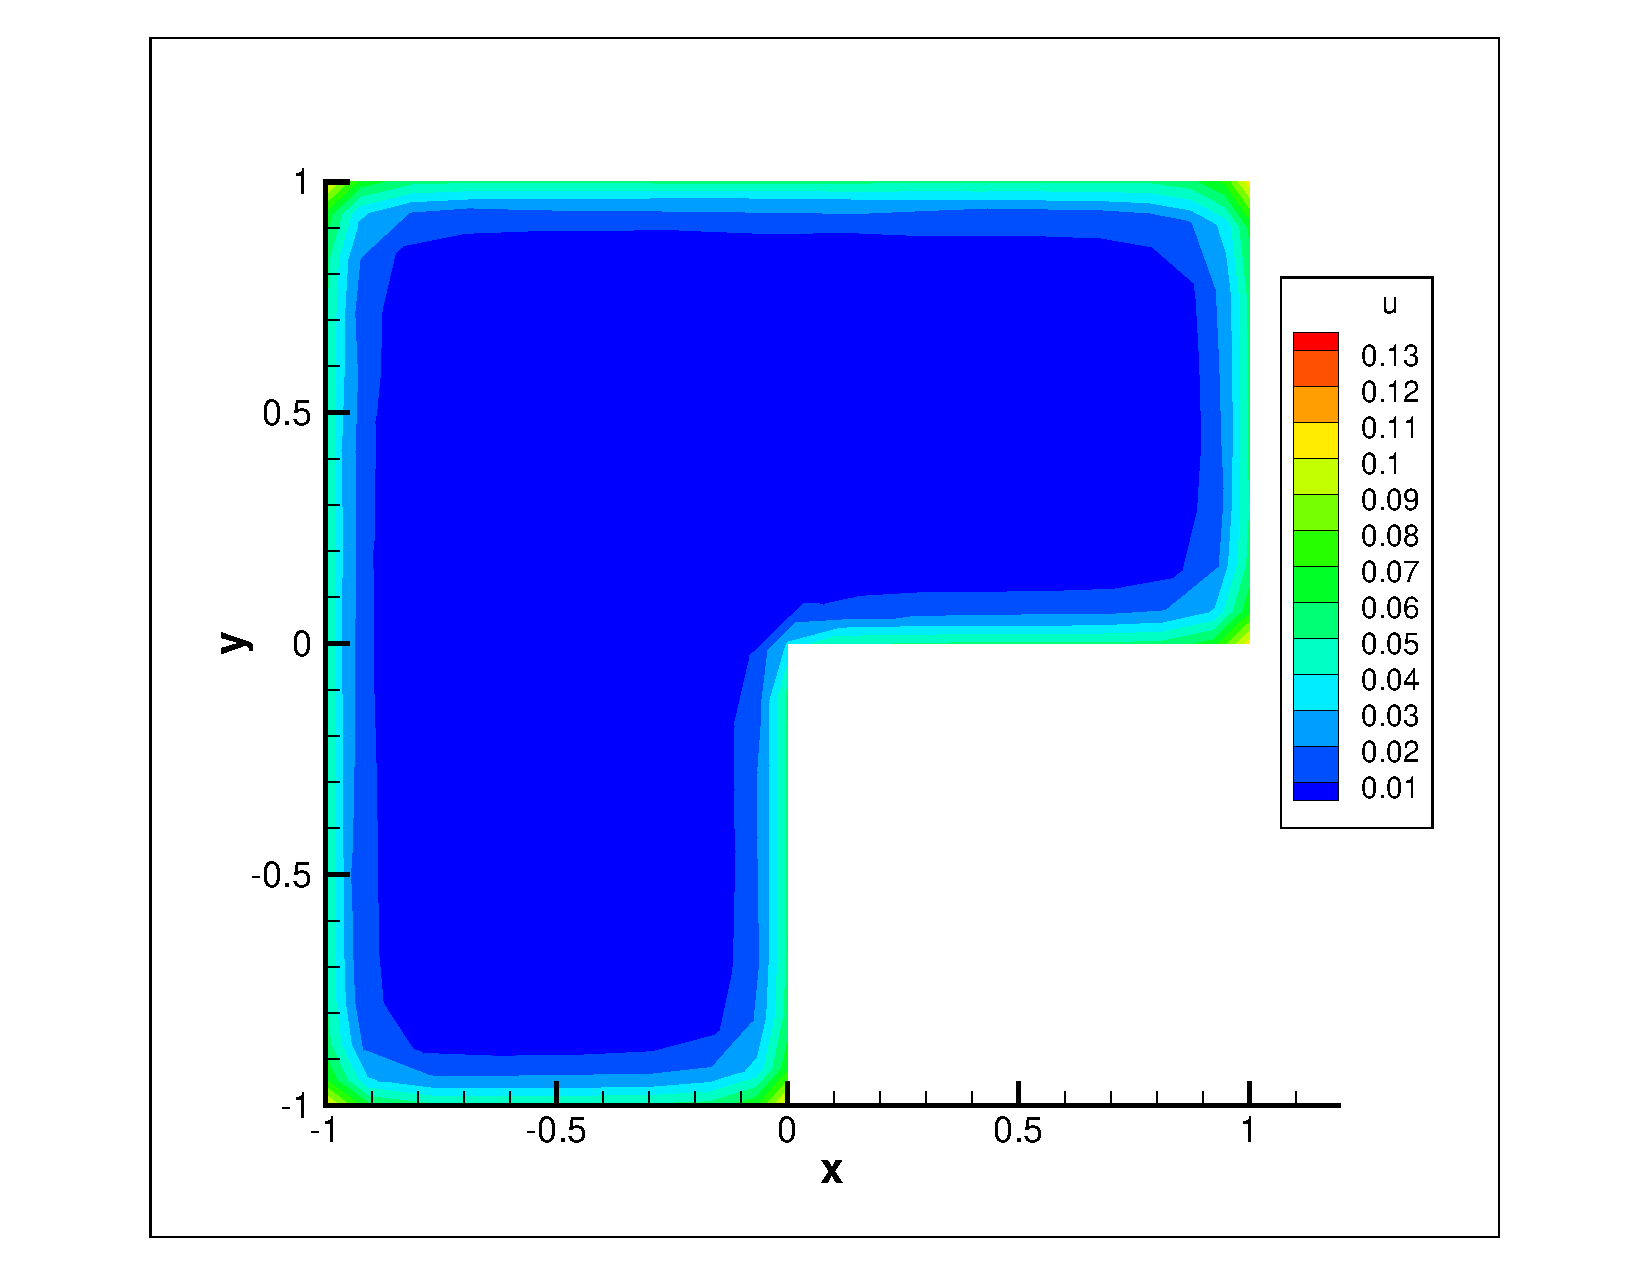
\includegraphics[viewport=110 30 600 520,clip=true,width=.42\textwidth]{figs/ly_redist_14_sol.pdf}}
%           \label{fig:ly_over}
%         \end{center}
%       \end{figure}
%   \end{itemize}
% }
